\section{Qu’est-ce qu’un graph}
Un graphe est un modèle abstrait de dessins de réseaux reliant des objets [b.8]. Ces modèles sont constitués par la donnée de sommets (aussi appelés nœuds), et d'arêtes (aussi appelées liens ou relation) entre ces sommets ; ces arêtes sont parfois non-symétriques (les graphes sont alors dits orientés) et sont appelés des flèches.\\

\begin{figure}[H]  
  \centering
    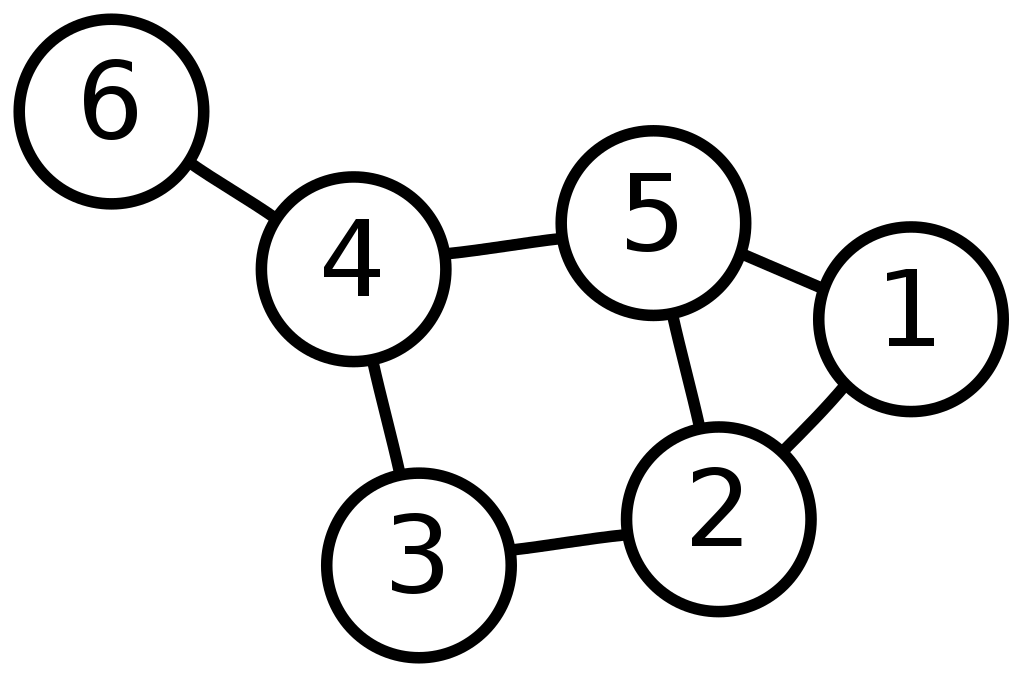
\includegraphics[width=0.5 \textwidth]{chapitre2/Figures/GraphNonOriontee.png}
  \caption{Graphe non orientée}
  \centering
    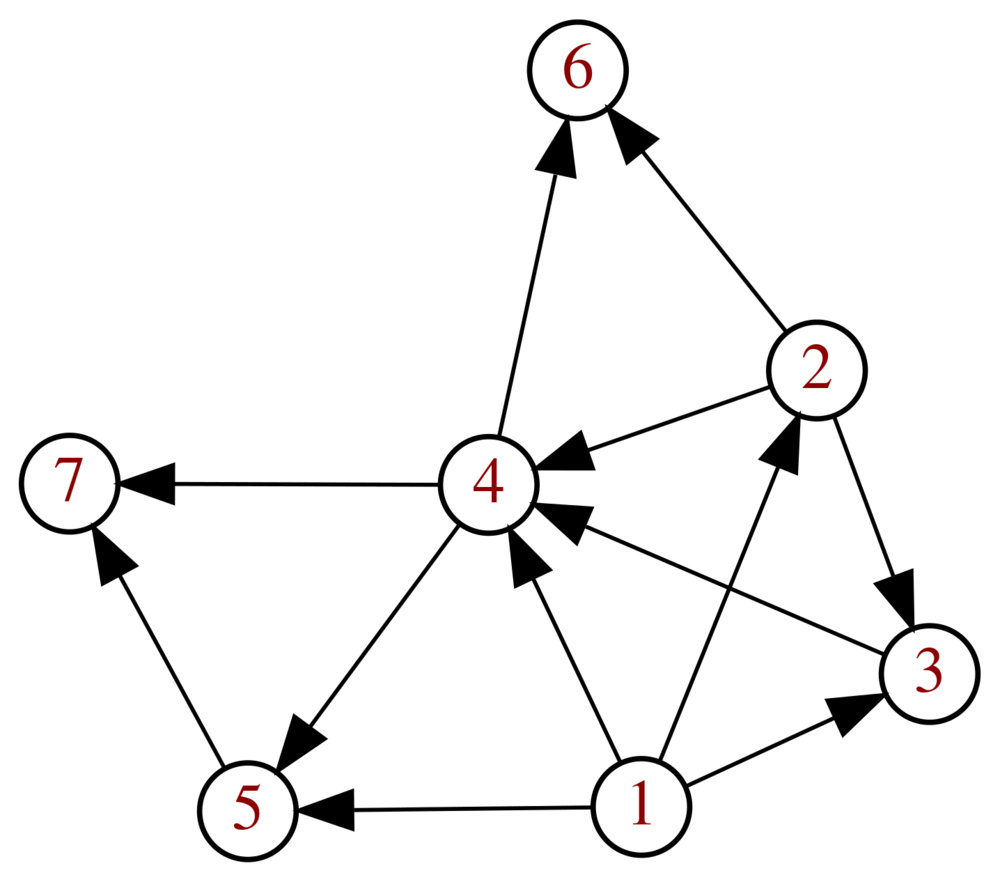
\includegraphics[width=0.5 \textwidth]{chapitre2/Figures/GraphOriontee.png}
  \caption{Graphe orientée}
\end{figure}

On ne peut pas parler des graphes dans le contexte académique sans parler de la théorie des graphes, c’est la discipline mathématique et informatique qui étudie les graphes. La théorie des graphes il a comme origine le mathématicien suisse Leonhard Euler, qui en 1735 a présenté à l'Académie de Saint-Pétersbourg un article qui traitait le problème des sept ponts de Königsberg. Le problème consistait à traverser une ville appelée Königsberg, cette ville est construite autour de deux îles situées sur un fleuve et reliées entre elles par un pont. Six autres ponts relient les rives de la rivière à l'une ou l'autre des deux îles, comme représentés dans la figure ci dessus. Le problème consiste à déterminer s'il existe ou non une promenade dans les rues de Königsberg permettant, à partir d'un point de départ au choix, de passer une et une seule fois par chaque pont, et de revenir à son point de départ, étant entendu qu'on ne peut traverser la rivière qu'en passant sur les ponts.\\

\begin{figure}[H]  
  \centering
    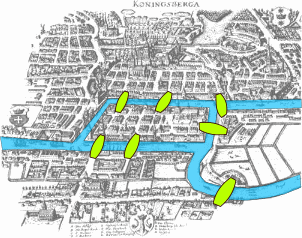
\includegraphics[width=0.4 \textwidth]{chapitre2/Figures/Konigsberg_bridges.png}
  \caption{Ville de Königsberg et ces sept ponts}
  \centering
    \includegraphics[width=0.4 \textwidth]{chapitre2/Figures/Königsberg_graph.svg.png}
  \caption{Modéle en graphe orionté de la ville de Königsberg}
\end{figure}

Les algorithmes élaborés pour résoudre des problèmes concernant les objets de cette théorie ont de nombreuses applications dans tous les domaines liés à la notion de réseau (réseau social, réseau informatique, télécommunications, etc.) et dans bien d'autres domaines.